%%
%% Copyright 2007, 2008, 2009 Elsevier Ltd
%%
%% This file is based on part of the 'Elsarticle Bundle'.
%% ---------------------------------------------
%%
%% It may be distributed under the conditions of the LaTeX Project Public
%% License, either version 1.2 of this license or (at your option) any
%% later version.  The latest version of this license is in
%%    http://www.latex-project.org/lppl.txt
%% and version 1.2 or later is part of all distributions of LaTeX
%% version 1999/12/01 or later.
%%
%% The list of all files belonging to the 'Elsarticle Bundle' is
%% given in the file `manifest.txt'.  Contact Elsevier for this file.
%%

%% Template article for Elsevier's document class `elsarticle'
%% with harvard style bibliographic references
%% SP 2008/03/01 
%%
%% $Id: elsarticle-template-harv.tex 4 2009-10-24 08:22:58Z rishi $
%%
%% This template is based on the 'elsarticle-template-harv.tex', but has been modified for specific use with submissions to the journal Ultrasound in Medicine and Biology, June 2010, KJH
%

% Use this set of document class options for submission
\documentclass[preprint,5p]{elsarticle}

% Use this set of document class options to obtain an approximate 2 column view, note that this is primarily intended to allow authors to determine line breaks for long equations.  It is NOT meant to identically reproduce how the article would look in print.
%\documentclass[3p,twocolumn,authoryear,12pt]{elsarticle}


%% if you use PostScript figures in your article
%% use the graphics package for simple commands
%% \usepackage{graphics}
%% or use the graphicx package for more complicated commands
%% \usepackage{graphicx}
%% or use the epsfig package if you prefer to use the old commands
%% \usepackage{epsfig}

%% The amssymb package provides various useful mathematical symbols
\usepackage{amssymb}
%% The amsthm package provides extended theorem environments
%% \usepackage{amsthm}

%% The lineno packages adds line numbers. Start line numbering with
%% \begin{linenumbers}, end it with \end{linenumbers}. Or switch it on
%% for the whole article with \linenumbers after \end{frontmatter}.
 \usepackage{lineno}
 
 %% The multirow package adds the ability to do multirow and 
 %% multicolumn spanning in LaTeX.  This package is used 
 %% as an example for this template in the tables section.
 \usepackage{multirow}

\journal{Ultrasound in Medicine and Biology}

\begin{document}

\begin{frontmatter}

%% Title

%% use the tnoteref command within \title for footnotes;
%% use the tnotetext command for the associated footnote;
%%
%% \title{Title\tnoteref{label1}}
%% \tnotetext[label1]{}
%% \author{Name\corref{cor1}\fnref{label2}}
%% \ead{email address}
%% \ead[url]{home page}
%% \fntext[label2]{}
%% \cortext[cor1]{}
%% \address{Address\fnref{label3}}
%% \fntext[label3]{}

\title{Acoustic Shadow Detection From Scanline Statistics of B-Mode or Radiofrequency Ultrasound Images}


%% Authors and addresses/affiliations

%% use the fnref command within \author or \address for footnotes;
%% use the fntext command for the associated footnote;
%% use the corref command within \author for corresponding author footnotes; note the corresponding author can be any of the authors, but one author must be designated; here the third author has been arbitrarily designated as the corresponding author as an example.
%% use the cortext command for the associated footnote;
%% use the ead command for the email address,
%% and the form \ead[url] for the home page:

%% \author{Name\corref{cor1}\fnref{label2}}
%% \ead{email address}
%% \ead[url]{home page}
%% \fntext[label2]{}
%% \cortext[cor1]{}
%% \address{Address\fnref{label3}}
%% \fntext[label3]{}

%% use optional labels to link authors explicitly to addresses:
%% \author[label1,label2]{<author name>}
%% \address[label1]{<address>}
%% \address[label2]{<address>}

\author[Affil1]{Ricky Hu}
\author[Affil2]{Rohit Singla}
\author[Affil1]{Farah Deeba \corref{cor1}}

\address[Affil1]{Robotics and Control Laboratory, Department of Electrical and Computer Engineering, University of British Columbia, Vancouver, Canada}
% Replace capitalized text with the appropriate information (use standard capitalization rules for your text, not all capitals.
\cortext[cor1]{Corresponding Author: Ricky Hu, Robotics and Control Laboratory, University of British Columbia, Room 3090, 2332 Main Mall, Vnacouver, BC, Canada V6T 1Z4.  Email: rhu@ece.ubc.ca}


\begin{abstract}
An acoustic shadow is an ultrasound image artifact that occurs in boundaries between significantly different material, such as tissue-bone or air-tissue boundaries, resulting in a continuous dark region on the image. Detection of shadow is important as shadows can identify anatomical features or may obscure regions of interests and images may be misinterpreted. A shadow detection method was developed by analyzing the statistics of patches of radiofrequency (RF) data. A second method was developed for brightness-mode (B-mode) images if RF data is unavailable by analyzing the cumulative entropy along interpolated scanline paths. Both methods utilized adaptive thresholding, needing only the pulse width of the transducer as an input parameter for easy utilization by different operators or equipment. Dice coefficients of X and X were obtained for the RF and B-mode methods, which is within range of the gold standard of manual detection on two different transducers and three different imaging locations. The results indicate that the methods are able to detect shadows with high versatility in different imaging scenarios. The method has the potential to aid interpretation of ultasound images or serve as an important pre-processing step for machine learning methods.
\end{abstract}


\begin{keyword}
%% keywords here, in the form: keyword \sep keyword.  You may use no more than 10 keywords.
Acoustic Shadow \sep Ultrasound \sep Speckle
\end{keyword}

\end{frontmatter}

%% Do not remove the page break here.
\pagebreak

\linenumbers

%% MAIN TEXT INSTRUCTIONS

%% For all sections, subsections, and subsubsections, use the '*' to remove numbering, as demonstrated below.

%% Commands for figures and tables should not be included in the main body of the submitted version of this file (e.g. the figure and tabular environments).  Figure captions should be listed in this file, as shown below.  Tables and Table captions should be listed as a separate section at the end of this file, as shown below.  Many authors may wish to include figures and tables within the main text of their document will preparing their manuscript.  This may be done, however please comment out any of the lines prior to submission.

%% Because the Elsevier editorial process does not allow for the figure and tabular environments in the submitted document, you will be unable to use autonumbering (i.e. \label and \ref) for figures and tables. 

%%  If long equations are used in the document, authors should use a two column format to make sure that the equations will break at approximately the right places.  To do this, replace the class option 'review' with the following two class options '3p' and 'twocolumn'.  Keep in mind that the column width produced in '3p' is slightly narrower than the final printer version.  After inserting the appropriate line breaks in your equation, change the '3p' option back to 'review'.

%% For citations, use the commands \citep and \citet

%% BEGIN MAIN TEXT

%%%%%%%%%%% INTRODUCTION
\section*{INTRODUCTION}
\label{intro}
Ultrasound devices have become increasingly affordable and portable, encouraging applications such as point-of-care ultrasound, novice usage, and data collection for machine learning. However, ultrasound is susceptible to unique artifacts that increase the difficult of interpretation and processing of images. One artifact is an acoustic shadow, which occurs when an ultrasound wave propagates from the transducer to a boundary of two materials with high impedance differences. The wave is almost completely reflected and beyond the boundary is a continuous dark region and a total loss of anatomical features. Acoustic shadows occur in air-tissue, tissue-bone, and tissue-lesion interfaces. Shadows can aid interpretation, such as identifying the presence of a gall stones or spinal level. However, shadows, such as from poor transducer contact, can lead to misinterpretation of anatomy, particularly by novice users and automated processing algorithms. Thus, the identification of shadows is an important preprocessing step in many applications.

Several methods have been used in literature to detect shadows. Geometric techniques model the path of an ultrasound signal for an expected image along the scanline using a random walk. Regions are then flagged as a shadow if a pixel is below a confidence threshold. However, geometric techniques require knowledge of the ultrasound transducer properties to assign weights to a random walk, such as the focal length, radius of curvature, and thickness. The technique would be cumbersome to implement across different ultrasound machines, especially if the source of the ultrasound images are unknown. This reduces the data available for machine learning applications and requires accurate transducer parameter labels for each image.

Pixel intensity methods ignore the properties of the transducer an analyze only the graphical properties of the image. Shadows have been detected on brain images by analyzing the entropy along a scanline to flag pixels of sudden low intensity as a potential shadow. The technique achieved a comparable Dice similarity coefficient as geometric methods but require specific thresholding, window sizing, filtering, and image mask parameterization for different anatomy. This method would be unfeasible in a clinical setting, particularly for novice users or point-of-care applications, as parameterization requires image processing expertise.

Machine learning methods have gained significant interest in medical imaging analysis although to our knowledge, no machine learning method has demonstrated capability of detecting shadows from multiple anatomy. Deep learning methods have been demonstrated to identify features in a common image set that contains a shadow, such as neuroanatomical regions in cranial scan or spinal levels in a posterior scan. Although machine learning has the potential of providing automated feature recognition in multiple applications, a large data set is required for an algorithm to recognize certain features. Ultrasound imaging is highly variable due to unique artifacts, operator technique, and equipment. In addition, shadows occur in various anatomy. Previous techniques focus on a single anatomical region and training data was from a consistent imaging scenario. However, it is difficult to construct a training data set with the generality required to recognize shadows in different scenarios usable for a variety of ultrasound applications.

We present a method utilizing radiofrequency (RF) or brightness-mode (B-mode) data that can detect shadows from multiple anatomy or transducers with minimum user configuration required. 

%%%%%%%%%%% MATERIALS AND METHODS
\section*{METHODS}
\label{MaM}
     
\subsection*{Data Collection}
Ultrasound RF and B-mode data was acquired by scanning 37 adult participants with informed written consent, approved by the University of British Columbia Research Ethics Board (Study ID: H18-01199). The scans included a forearm scan near the distal end of the pronator quadratus, an elbow scan near the cubital fossa, and a rib scan on the anterior surface of right ribs 11-12. Each scan was taken with both a curvilinear (C5-2/60, Ultrasonix, Canada) and linear (L14-5/38, Ultrasonix, Canada) transducer. Different transducer settings were used for each anatomical region and transducer, summarized in Table 1. The experiment was designed to generate a dataset from various imaging scenarios to validate the versatility of the shadow detection method.


\begin{table}[]
	\begin{tabular}{|l|l|l|l|l|}
		\hline
		\textbf{}                                                                                              & \textbf{Anatomy} & \textbf{Frequency} & \textbf{Depth} & \textbf{Gain} \\ \hline
		\multirow{3}{*}{\textbf{\begin{tabular}[c]{@{}l@{}}Linear\\ Transducer\\ (L14-5/38)\end{tabular}}}     & Forearm          & 11.0MHz            & 5.0cm          & 50\%          \\ \cline{2-5} 
		& Elbow            & 11.0MHz            & 5.0cm          & 40\%          \\ \cline{2-5} 
		& Ribcage          & 5.0MHz             & 10.0cm         & 30\%          \\ \hline
		\multirow{3}{*}{\textbf{\begin{tabular}[c]{@{}l@{}}Curvilinear\\ Transducer\\ (C5-2/60)\end{tabular}}} & Forearm          & 4.0MHz             & 5.0cm          & 50\%          \\ \cline{2-5} 
		& Elbow            & 4.0MHz             & 5.0cm          & 40\%          \\ \cline{2-5} 
		& Ribcage          & 3.3MHz             & 10.0cm         & 30\%          \\ \hline
	\end{tabular}
\end{table}


\subsection*{Radiofrequency Speckle Analysis}      
To detect shadows, patches of speckle was analyzed on the RF signal. Speckle occurs due to multiplicative scattering of acoustic waves in a material, resulting in a granular patch on the image. B-mode data commonly attempts to remove speckle, but speckle contains information of the acoustic interactions in tissue. Speckle can then characterize different regions, such as a region of tissue or a region of signal loss in a shadow. In addition, B-mode data can be manipulated by an operator to visually enhance an image, such as adjusting time-gain compensation or dynamic range. Thus, speckle analysis can provide a more robust shadow detection usable across different machines and operators.

One of the first models for speckle is with a one-parameter Rayleigh distribution to model the probability density of a random walk. The Rayleigh is capable for modeling fully developed speckle, which does not occur when there is limited scattering. More generalized models have been applied such as the Rician, Homodyned-K, and Nakagami distributions to characterize general speckle. Speckle has been leveraged to analyze features such as classifying tumorigenicity of breast lesions or levels of liver fibrosis. Shadow detection presents a simpler problem than comparing regions of similar tissue as a shadow and non-shadow region contain significantly different speckle patterns. Thus, the Nakagami distribution expressed in Eq. 1 was chosen to model speckle. The Nakagami distribution provides greater generality than the Rayleigh distribution while being more computationally efficient than the Rician or Homodyned K distributions.

\begin{equation}
\Phi(x,\mu,\omega) = 2(\frac{\mu}{\omega})^{\mu}\frac{1}{\Gamma(\mu)}x^{(2\mu-1)}e^{\frac{-\mu}{\omega}x^{2}}
\end{equation}

Where $x$ is the RF intensity, $\mu$ is the shape parameter, $\omega$ is the scale parameter and $\Gamma(\mu)$ is the gamma distribution.

To detect shadows, the raw RF data was first processed by computing the echo envelope of each scanline with a Hilbert transform. An absolute logarithmic scale of the echo envelope was taken to generate an "RF Image", which is visually similar to B-mode without filtering to remove artifacts. Next, the RF image was divided into overlapped patches with a width of a single RF data point and a length of three times the pulse width. This patch size was demonstrated in literature to be sufficiently large to capture multiple wavelengths and scattering events while being small enough to be useful in differentiating different regions on the millimeter scale. Next, the RF data in each patch was fit to a Nakagami distribution using a maximum likelihood estimate to compute the fitted Nakagami shape and scale parameters $\mu$ and $\omega$, producing a map of Nakagami parameter values for an image as shown in Fig. 1.

\begin{figure}
	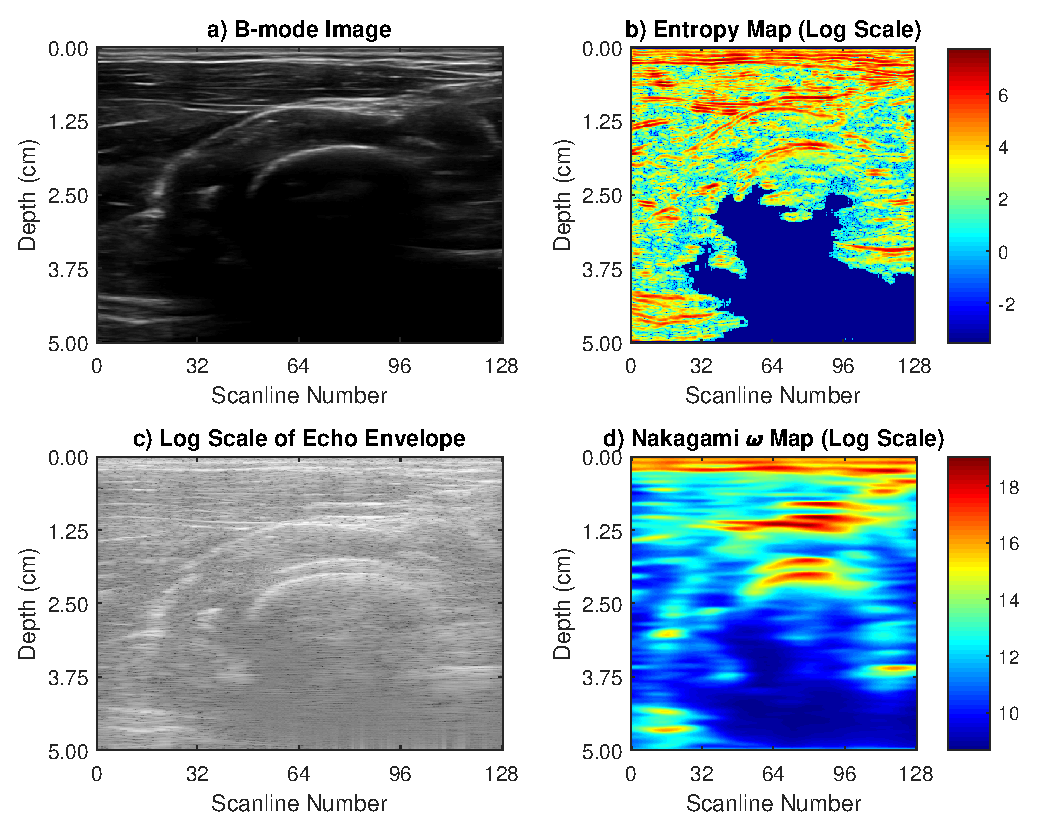
\includegraphics[scale=0.5]{fig2.pdf}
\end{figure}

Since the Nakagami distributions are significantly different for shadow regions with abundant speckle and non-shadow regions with minimal speckle, a simple automated thresholding scheme was used. Otsu's method was applied on the entire image to compute a threshold for the Nakagami parameters. Then, for each scanline, the deepest data point that is above the threshold is labeled as the shadow boundary and all data points below are labeled as a shadow.

\subsection*{B-mode Scanline Analysis}

Many ultrasound machines do not provide access to RF data needed for speckle analysis. Thus, we present a shadow detection method on B-mode images that addresses the need for usability across different equipment with minimum configuration. First, the cumulative scanline entropy is computed for each pixel, which is similar to the "Rupture Criterion" developed by Hellier et al., with the window size fixed as three times the pulse width, $\eta$, as defined in Eq. 2

\begin{equation}
S_{i,j} = \sum_{i=1}^{3\eta}I(i-1)log_{2}\frac{I(i-1)}{I(i+1)}+I(i+1)log_{2}\frac{I(i+1)}{I(i-1)}  \forall i \exists L
\end{equation}

Where $S_{i,j}$ is the cumulative entropy at pixel $i$ on scanline $j$, $\eta$ is the pulse width, $I(i)$ is the pixel intensity of pixel $i$, and $L$ is the set of scanline elements that are not the first or last element.

Note that for linear images, tracking the scanlines is simple. For curvilinear images, the scanline paths were tracked by first capturing the slope of the lateral edges by following the ring-down regions. Ring-down is a consistent artifact that produces bright bands at the top of an image due to the fluid in the transducer reflecting a continuous signal. The scanlines were then interpolated between the slopes of the lateral edges.

Next, Otsu's method is applied similarly to compute a threshold entropy value. The intuition of the threshold is different than in RF analysis. In RF analysis, the threshold separates patches of intense and minimal speckle. In B-mode analysis, the threshold separates pixels of a shadow boundary, which has high entropy, and pixels of non-boundaries, which include shadow and non-shadow regions. Thus, shadows can be identified by finding the last pixel on a scanline with an entropy higher than the threshold, representing a bright shadow boundary.



\subsection*{Validation}

A trained annotator manually outlined shadow regions on B-mode images. The manual regions were used as a gold standard, as manual identification is common in clinical practice and has been used in previous literature for comparison. A dice coefficient was computed to compare similarity of manual and automated shadow detection.

%%%%%%%%%%% Results
\section*{Results}
\label{Results}

Examples of detected shadows from both methods are highlighted in gray in Fig. 2 in different imaging scenarios.

\begin{figure}
	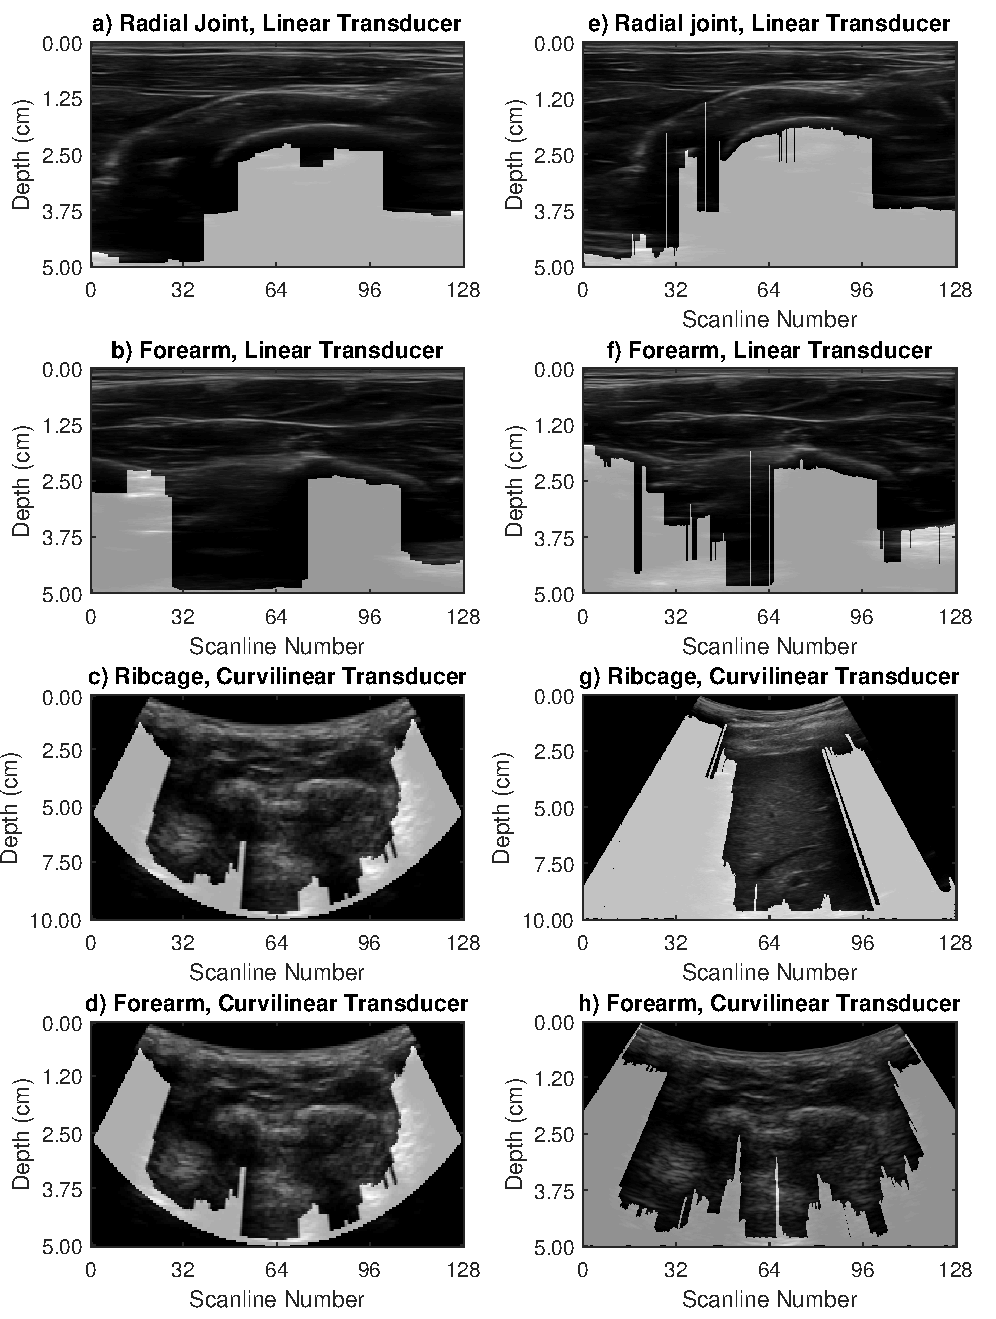
\includegraphics[scale=0.55]{fig1.pdf}
\end{figure}

The Dice coefficients for both methods for different anatomy and trasducers are shown in Table 2. 

\begin{table}[]
	\begin{tabular}{|l|l|l|l|}
		\hline
		\textbf{}                                                                                 &         & \textbf{RF} & \textbf{B-Mode} \\ \hline
		\multirow{3}{*}{\begin{tabular}[c]{@{}l@{}}Linear\\ Transducer\\ (L14-5/38)\end{tabular}} & Forearm & x                   & x                             \\ \cline{2-4} 
		& Elbow   & x                   & x                             \\ \cline{2-4} 
		& Ribcage & x                   & x                             \\ \hline
		\multirow{3}{*}{Curvilinear Transducer}                                                   & Forearm & x                   & x                             \\ \cline{2-4} 
		& Elbow   & x                   & x                             \\ \cline{2-4} 
		& Ribcage & x                   & x                             \\ \hline
	\end{tabular}
\end{table}

%%%%%%%%%%% DISCUSSION
\section*{Discussion}
\label{Discuss}
Previous studies reported that the Dice coefficient between manual annotators recorded a mean of X . Every scenario detected from both methods achieved a Dice coefficient within the range of manual detection. This supports the versatility of the detection method as both methods are able to identify shadows across different anatomy and transducers with minimum configuration. 

However, the inconsistency of manual detection presents two problems. One is that by using a subjective gold standard with Dice upper bound below 1.0, it is difficult to compare the performance of different algorithms. Secondly, the inconsistency of manually identified shadows reflect on the lack of a clear definition for a shadow. In images with a shadow, such as in Fig. 2 a), the shadow boundary of the radial joint appears as a bright arc. Looking closely at the scanline of the boundary, the pixels first increase in brightness and then decrease before becoming a clear, dark shadow. There is no consensus as to where the shadow begins, whether it is the brightness point on the scanline or when the signal drops below a threshold. Thus, there a limitation on validation and this work focused on improving the versatility and usability of shadow detection while maintaining similar accuracy as previous methods.

%%%%%%%%%%% Conclusions
\section*{Conclusions}
\label{Conclusions}
Two methods were developed for acoustic shadow detection requiring only the transducer pulse width as the input parameter. When comparing to manual detection, the methods achieved a Dice similarity coefficient above X for three different anatomical locations and two different transducers, indicating high similarity. The versatility of the shadow detection method has potential to improve the interpretation of ultrasound images with shadow artifacts or to serve as a pre-processing step for machine learning methods in the future.
        
%%%%%%%%%%% ACKNOWLEDGEMENTS
\section*{Acknowledgements}
\label{Ack}
Type in any acknowledgements here.  If there are no acknowledgments, please delete or comment out this section.



%% The Appendices part is started with the command \appendix;
%% appendix sections are then done as normal sections
%% \appendix

%% \section*{}
%% \label{}


%%%%%%%%%%% REFERENCES
%% REFERENCE FORMATTING INSTRUCTIONS

%% All bibliography information should be included using a 'thebibliography' environment.  Most authors will find it easiest to create a .bbl file using the commands \bibliographystyle{} and \bibliography{} and then copy and paste the contents of the .bbl file into the .tex file below, but before the figure captions section.  Examples for using the \bibliographystyle and \bibliography commands are listed below.  

%% Do not remove the page break here.
\pagebreak

%% References with bibTeX database, use this to create a .bbl file
%\bibliographystyle{UMB-elsarticle-harvbib}
%\bibliography{FILENAME_OF_YOUR_BIBTEX_DATABASE}

%% References copied and pasted from the .bbl file.  Copy and paste over the following two lines.  When using a bibTeX database to create a .bbl file, comment out the following two lines.
\begin{thebibliography}{00}
\end{thebibliography}

%%%%%%%%%%% FIGURE CAPTIONS

%% Include only the figure captions here (not the figures).  Figures are uploaded separately in the online Elsevier Editorial Submission process.

%% Do not remove the page break here.
\pagebreak

\section*{Figure Captions}

\begin{description}
\item[Figure 1:]  TYPE THE CAPTION FOR FIGURE ONE HERE.
\item[Figure 2:]  TYPE THE CAPTION FOR FIGURE TWO HERE.
\item[Figure 3:]  TYPE THE CAPTION FOR FIGURE ONE HERE.  CONTINUE THIS LIST FOR ALL OTHER CAPTIONS
\end{description}

%%%%%%%%%%% TABLES AND TABLE CAPTIONS

%% Both tables and table captions should be included below.  Captions should appear above the table, as shown below. If users want to use multirow.sty, array.sty, etc., to fine control/enhance the tables, they are welcome to load any package of their choice and the elsearticle.cls should work in combination with all loaded packages.  For problems with loaded packages please contact: elsarticle@river-valley.com (the developers of the elsarticle document class) or support@elsevier.com (Elsevier customer support).

%% Since the tabular format is often difficult to work with for complex tables, authors may also choose to create their tables with another program.  Each table and it's corresponding caption should then be saved as a pdf.  Each pdf should then be uploaded separately during the online submission process.  If doing so, all of the text below concerning tables and table captions should be commented out.

%% If no tables are part of the manuscript, comment out or delete this entire section.

%% Do not remove the page break here.
\pagebreak


%%%%%%%%%%% VIDEO CAPTIONS

%% If submitting video's as a supplement to the manuscript, include only the video captions here (not the figures).  Videos are uploaded separately in the online Elsevier Editorial Submission process.  If videos are not included, comment out this section.

%% Do not remove the page break here.
\pagebreak





\end{document}
